% PRL look and style (easy on the eyes)
\documentclass[aps,pre,twocolumn,nofootinbib,superscriptaddress,linenumbers]{revtex4-1}
% Two-column style (for submission/review/editing)
%\documentclass[aps,prl,preprint,nofootinbib,superscriptaddress,linenumbers]{revtex4-1}

\pdfoutput=1
\usepackage[pdftex]{graphicx}

\usepackage{alltt}
\usepackage{fancyvrb}


%\usepackage{palatino}

%\usepackage{palatino}
% Change to a sans serif font.
\usepackage{sourcesanspro}
\renewcommand*\familydefault{\sfdefault} %% Only if the base font of the document is to be sans serif
\usepackage[T1]{fontenc}
%\usepackage[font=sf,justification=justified]{caption}
\usepackage[font=sf]{floatrow}

% To allow code "Boxes" as well as figures
\usepackage{newfloat}
\DeclareFloatingEnvironment[name={Box}]{codebox}

% Rework captions to use sans serif font.
\makeatletter
\renewcommand\@make@capt@title[2]{%
 \@ifx@empty\float@link{\@firstofone}{\expandafter\href\expandafter{\float@link}}%
  {\sf\textbf{#1}}\sf\@caption@fignum@sep#2\quad
}%
\makeatother

\usepackage{listings} % For code examples
\usepackage[usenames,dvipsnames,svgnames,table]{xcolor}

\usepackage{amsmath}
\usepackage{amssymb}
%\usepackage[mathbf,mathcal]{euler}
%\usepackage{citesort}
\usepackage[caption=false]{subfig}
\usepackage{dcolumn}
\usepackage{boxedminipage}
\usepackage{verbatim}
\usepackage[colorlinks=true,citecolor=blue,linkcolor=blue]{hyperref}
\usepackage[group-separator={,}]{siunitx}
\usepackage{booktabs}

% Justification
\captionsetup{singlelinecheck=off}

% Pretty-printing of shell commands
\newcommand{\shellcmd}[1]{\\\ \texttt{\scriptsize #1}}

% The figures are in a figures/ subdirectory.
\graphicspath{{../figures/}}

%% DOCUMENT %%%%%%%%%%%%%%%%%%%%%%%%%%%%%%%%%%%%%%%%%%%%%%%%%%%%%%%%%%%%%%%%%%%%
\begin{document}

%% TITLE %%%%%%%%%%%%%%%%%%%%%%%%%%%%%%%%%%%%%%%%%%%%%%%%%%%%%%%%%%%%%%%%%%%%
\title{An open library of human kinase domain constructs for automated bacterial expression}

\author{Daniel L. Parton}
  \affiliation{Computational Biology Program, Sloan Kettering Institute, Memorial Sloan Kettering Cancer Center, New York, NY 10065}
  \email{daniel.parton@choderalab.org}
\author{Sonya M. Hanson}
  \affiliation{Computational Biology Program, Sloan Kettering Institute, Memorial Sloan Kettering Cancer Center, New York, NY 10065}
  \email{sonya.hanson@choderalab.org}
\author{Lucelenie Rodr�guez-Laureano}
  \affiliation{Computational Biology Program, Sloan Kettering Institute, Memorial Sloan Kettering Cancer Center, New York, NY 10065}
  \email{lucelenie.rodriguez@choderalab.org}
\author{Steven K. Albanese}
  \affiliation{Gerstner Sloan Kettering Graduate School, Memorial Sloan Kettering Cancer Center, New York, NY 10065}
  \email{steven.albanese@choderalab.org}
\author{Scott Gradia}
  \affiliation{QB3 MacroLab, University of California, Berkeley, CA 94720}
  \thanks{Current address: Caribou Biosciences, Berkeley, CA 94720}
  \email{sgradia@cariboubio.com}
\author{Chris Jeans}
  \affiliation{QB3 MacroLab, University of California, Berkeley, CA 94720}
  \email{c.jeans@berkeley.edu}
\author{Markus Seeliger}
\affiliation{Department of Pharmacological Sciences, Stony Brook University Medical School, Stony Brook, NY 11794}
\email{markus.seeliger@stonybrook.edu}
\author{John D. Chodera}
 \thanks{Corresponding author}
 \email{john.chodera@choderalab.org}
  \affiliation{Computational Biology Program, Sloan Kettering Institute, Memorial Sloan Kettering Cancer Center, New York, NY 10065}

\date{\today}

%%%%%%%%%%%%%%%%%%%%%%%%%%%%%%%%%%%%%%%%%%%%%%%%%%%%%%%%%%%%%%%%%%%%%%%%%%%%%%%%%%%%%%%%%%%%%%%%%%%%%%
% ABSTRACT/pacs
%%%%%%%%%%%%%%%%%%%%%%%%%%%%%%%%%%%%%%%%%%%%%%%%%%%%%%%%%%%%%%%%%%%%%%%%%%%%%%%%%%%%%%%%%%%%%%%%%%%%%%
\begin{abstract}
Kinases play a critical role in cellular signaling pathways.
Human kinase dysregulation linked to a number of diseases, such as cancer, diabetes, and inflammation, and as a result, much of the effort in developing treatments (and perhaps 30\% of \emph{all} current drug development effort) has focused on shutting down aberrant kinases with targeted inhibitors.
While insect and mammalian expression systems have demonstrated success rates for the expression of human kinases, these expression systems cannot compete with the simplicity and cost-effectiveness of bacterial expression systems, which historically had found human kinases difficult to express.
Following the demonstration that phosphatase coexpression could give high yields of Src and Abl kinase domains in inexpensive bacterial expression systems~\cite{seeliger:2005:protein-sci:kinase-expression}, we have performed a large-scale expression screen to generate a library of human kinase domain constructs that express well in a simple automated His-tagged bacterial expression system when coexpressed with phosphatase (YopH for Tyr kinases, lambda for Ser/Thr kinases).
Starting from 96 kinases with crystal structures and any reported bacterial expression, we engineered a library of human kinase domain constructs and screened their coexpression with phosphatase, finding 68 kinases with yields greater than 2  mg/mL culture.
All sequences and expression data are provided online at  \url{https://github.com/choderalab/kinase-ecoli-expression-panel}, and the plasmids are in the process of being made available through AddGene.
\end{abstract}

\maketitle

%%%%%%%%%%%%%%%%%%%%%%%%%%%%%%%%%%%%%%%%%%%%%%%%%%%%%%%%%%%%%%%%%%%%%%%%%%%%%%%%%%%%%%%%%%%%%%%%%%%%%%
% INTRODUCTION
%%%%%%%%%%%%%%%%%%%%%%%%%%%%%%%%%%%%%%%%%%%%%%%%%%%%%%%%%%%%%%%%%%%%%%%%%%%%%%%%%%%%%%%%%%%%%%%%%%%%%%
\section{Introduction}
\label{section:introduction}

Kinases play a critical role in cellular signaling pathways.  
Perturbations to these pathways due to mutation, translocation, or upregulation events can cause one or more kinases to become highly active and cease responding normally to regulatory signals, often with disastrous consequences.
Kinase dysregulation has been linked to a number of diseases, such as cancer, diabetes, and inflammation.
Cancer alone is the second leading cause of death in the United States, accounting for nearly 25\% of all deaths; in 2015, over 1.7 million new cases were diagnosed, with over 580,000 deaths~\cite{acs-cancer-facts-2015}.
Much of the effort in developing treatments (and perhaps 30\% of \emph{all} current drug development effort) has focused on shutting down aberrant kinases with targeted inhibitors.

The discovery of imatinib, which specifically targets the Abl kinase dysregulated in chronic myelogenous leukemia (CML) patients to abate disease progression, was transformative in revealing the enormous therapeutic potential of selective kinase inhibitors, kindling hope that this remarkable success could be recapitulated for other cancers and diseases~\cite{stegmeier:clpt:2010:imatinib-lessons}.
While there are now 31 FDA-approved selective kinase inhibitors, these molecules were approved for targeting only 13 out of $\sim$500 human kinases, with the vast majority targeting just a handful of kinases; the discovery of therapeutically effective inhibitors for other kinases has proven remarkably challenging.

The ability to probe human kinase biochemistry, biophysics, and structural biology in the laboratory is essential to making rapid progress in the understanding of kinase regulation and the design of selective inhibitors.
While human kinase expression in baculovirus-infected insect cells can achieve high success rates~\cite{vertex:2004:kinase-expression,wang:protein-express-pur:2008:high-yield-kinase-insect-cells}, it cannot compete in cost or convenience with bacterial expression.
While a survey of 62 full-length non-receptor human kinases found that over 50\% express well in \emph{E. coli}~\cite{vertex:2004:kinase-expression}, there is often a desire to express and manipulate only the soluble kinase domains, since these are the molecular targets of therapy for targeted kinase inhibitors and could be studied even for receptor-type kinases.
While removal of regulatory domains can negatively impact expression, coexpression with phosphatase was shown to greatly enhance bacterial kinase expression in Src and Abl tyrosine kinases, presumably by ensuring that kinases remain in an unphosphorylated inactive form~\cite{seeliger:2005:protein-sci:kinase-expression}.

The protein databank (PDB) now contains over 100 human kinases that---according to the PDB data records---were expressed in bacteria.
Since bacterial expression is often complicated by the need to tailor expression and purification protocols individually for each protein expressed, we wondered whether a simple, uniform, automatable expression and purification protocol could be used to express a large number of human kinases to produce a convenient bacterial expression library to facilitate kinase research and selective inhibitor development.
As a first step toward this goal, we developed a structural informatics pipeline to find kinases already in the PDB and select constructs from available human kinase libraries to clone into a standard set of vectors intended for phosphatase coexpression.
Automated expression screening in ROSETTA2 [BL21(DE3)] cells found that 68 human kinase domains express with yields greater than 2 $\mu$g/mL, which should be usable for biochemical, biophysical, screening, and structural biology studies.

All code and source files used in this project can be found at \url{https://github.com/choderalab/kinase-ecoli-expression-panel}, and a convenient sortable table of results can be viewed at \url{http://choderalab.github.io/kinome-data/kinase\_constructs-addgene\_hip\_sgc.html}.

%%%%%%%%%%%%%%%%%%%%%%%%%%%%%%%%%%%%%%%%%%%%%%%%%%%%%%%%%%%%%%%%%%%%%%%%%%%%%%%%%%%%%%%%%%%%%%%%%%%%%%
% METHODS
%%%%%%%%%%%%%%%%%%%%%%%%%%%%%%%%%%%%%%%%%%%%%%%%%%%%%%%%%%%%%%%%%%%%%%%%%%%%%%%%%%%%%%%%%%%%%%%%%%%%%%
\section{Methods}
\label{section:methods}

\subsection{Semi-automated selection of kinase construct sequences for E. coli expression}

\subsubsection{Selection of human protein kinase domain targets}

Human protein kinases were selected by querying the UniProt API for any human protein with a domain containing the string "protein kinase", and which was manually annotated and reviewed (i.e. a Swiss-Prot entry).
The query string used was:\\
{\tt taxonomy:"Homo sapiens (Human) [9606]" AND domain:"protein kinase" AND reviewed:yes}\\
Data was returned by the UniProt API in XML format and contained protein sequences and relevant PDB structures, along with many other types of genomic and functional information.
To select active protein kinase domains, the UniProt domain annotations were searched using the regular expression {\tt \^{}Protein kinase(?!; truncated)(?!; inactive)}, which excludes certain domains annotated "Protein kinase; truncated" and "Protein kinase; inactive".
Sequences for the selected domains were then stored.
The sequences were derived from the canonical isoform as determined by UniProt.

\subsubsection{Matching target sequences with relevant PDB constructs}

Each target kinase gene was matched with the same gene in any other species where present, and UniProt data was downloaded for those genes also.
The UniProt data included a list of PDB structures which contain the protein, as well as their sequence spans in the coordinates of the UniProt canonical isoform.
This information was used to filter out PDB structures which did not include the protein kinase domain - structures were kept if they included the protein kinase domain sequence less 30 residues at each end.
PDB coordinate files were then downloaded for each PDB entry.
The coordinate files contain various metadata, including an {\tt EXPRESSION\_SYSTEM} annotation, which was used to filter PDB entries to keep only those which include the phrase "ESCHERICHIA COLI".
The majority of PDB entries returned had an {\tt EXPRESSION\_SYSTEM} tag of "ESCHERICHIA COLI", while a small number had "ESCHERICHIA COLI BL21" or "ESCHERICHIA COLI BL21(DE3).

The PDB coordinate files also contain SEQRES records, which should contain the protein sequence used in the crystallography or NMR experiment.
According to the PDB documentation (\url{http://deposit.rcsb.org/format-faq-v1.html}), "All residues in the crystal or in solution, including residues not present in the model (i.e., disordered, lacking electron density, cloning artifacts, HIS tags) are included in the SEQRES records."
However, we found that these records are very often misannotated, instead representing only the crystallographically resolved residues.
Since expression levels can be greatly affected by insertions or deletions of only one or a few residues at either terminus~\cite{klock_combining_2008}, it is important to know the full experimental sequence, and we thus needed a way to measure the authenticity of a given SEQRES record.
%{\color{blue}[DLP: ?CITE, or reference our 96-construct Abl1 expression panel]}
We developed a crude measure by hypothesizing that a) most crystal structures would be likely to have at least one or a few unresolved residues at one or both termini and b) the presence of an expression tag (which is typically not crystallographically resolved) would indicate an authentic SEQRES record.
To achieve this, unresolved residues were first defined by comparing the SEQRES sequence to the resolved sequence, using the SIFTS service to determine which residues were not present in the canonical isoform sequence.
%SIFTS service (CITE)
Then regular expression pattern matching was used to detect common expression tags at the N- or C-termini.
Sequences with a detected expression tag were given a score of 2, while those with any unresolved sequence at the termini were given a score of 1, and the remainder were given a score of 0.
This data was not used to filter out PDB structures at this stage, but was stored to allow for subsequent selection of PDB constructs based on likely authenticity.
Also stored for each PDB sequence was the number of residues extraneous to the target kinase domain, and the number of residue conflicts with the UniProt canonical isoform within that domain span.

\subsubsection{Plasmid libraries}

As a source of kinase DNA sequences, we purchased three kinase plasmid libraries: the \href{https://plasmid.med.harvard.edu/PLASMID/Home.xhtml}{addgene Human Kinase ORF kit }, a kinase library from the Structural Genomics Consortium (SGC), Oxford (\url{http://www.thesgc.org}), and a kinase library from the \href{https://plasmid.med.harvard.edu/PLASMID/Home.xhtml}{PlasmID Repository} maintained by the Dana-Farber/Harvard Cancer Center.
The aim was to subclone the chosen sequence constructs from these plasmids, though we did not use the same vectors.
Annotated data for the kinases in each library was used to match them against the human protein kinases selected for this project.
A Python script was written which translated the plasmid ORFs into protein sequences, and aligned them against the target kinase domain sequences from UniProt.
Also calculated were the number of extraneous protein residues in the ORF, relative to the target kinase domain sequence, and the number of residue conflicts.

\subsubsection{Selection of sequence constructs for expression}

Of the kinase domain targets selected from UniProt, we filtered out those with no matching plasmids from our available plasmid libraries and/or no suitable PDB construct sequences.
For this purpose, a suitable PDB construct sequence was defined as any with an authenticity score > 0, i.e. those derived from SEQRES records with no residues outside the span of the resolved structure.
Plasmid sequences and PDB constructs were aligned against each target domain sequence, and various approaches were then considered for selecting a) the sequence construct to use for each target, and b) the plasmid to subclone it from.
Candidate sequence constructs were drawn from two sources - PDB constructs and the SGC plasmid library.
The latter sequences were included because the SGC plasmid library was the only one of the three libraries which had been successfully tested for E. coli expression.

For most of the kinase domain targets, multiple candidate sequence constructs were available.
To select the most appropriate sequence construct, we sorted them first by authenticity score, then by the number of conflicts relative to the UniProt domain sequence, then by the number of residues extraneous to the UniProt domain sequence span.
The top-ranked construct was then chosen.
In cases where multiple plasmids were available, these were sorted first by the number of conflicts relative to the UniProt domain sequence, then by the number of residues extraneous to the UniProt domain sequence span, and the top-ranked plasmid was chosen.

This process resulted in a set of 96 kinase domain constructs, which (by serendipity) matched the 96-well plate format we planned to use for parallel expression testing.
We therefore selected these construct sequences for expression testing.

A sortable table of results can be viewed at \url{http://choderalab.github.io/kinome-data/kinase\_constructs-addgene\_hip\_sgc.html}.

%{
%\color{blue}
%TODO maybe include a figure to help illustrate the above (but may be too complicated):
% Get UniProt canonical isoform sequence
% Interested only in PK domain
% Then get relevant PDB structures - keep only those which include the PK domain less 30 residues at either end.
% ...
%}

\subsubsection{Other notes}

While much of this process was performed programmatically using Python, many steps required manual supervision and intervention.
We hope eventually to develop a fully automated software package for the selection of expression construct sequences for a given protein family, but this was not possible within the scope of this article.

\subsection{Expression testing}

%{\color{red}[JDC: This protocol is missing crucial information, like exactly which cell type was used for expression!]}

For each target, the selected construct sequence was subcloned from the selected DNA plasmid.
Expression testing performed by QB3 MacroLab.

All genes were cloned into the 2BT10 plasmid, an AMP resistant ColE1 plasmid with a T7 promoter.
Each kinase domain was tagged with a N-terminal His10-TEV and co-expressed with either the truncated YopH164 (for Tyr kinases) or lambda phosphatase (for Ser/Thr kinases). 
Expression was performed in Rosetta2 cells grown with Magic Media (Invitrogen autoinducing medium), 100 $\mu$g/mL of carbenicillin and 100 $\mu$g/mL of spectinomycin. 
Single colonies of transformants were cultivated with 900 $\mu$L of MagicMedia into a gas permeable sealed 96-well block. 
The cultures were incubated at 37$^\circ$C for 4 hours and then at 16 $^\circ$C for 40 hours while shaking. 
Next, cells were centrifuged and the pellets were frozen at -80 $^\circ$C overnight. 
Cells were lysed on a rotating platform at room temperature for an hour using 700 $\mu$L of SoluLyse (Genlantis) supplemented with 400 mM NaCl, 20 mM imidazole and protease inhibitors. 

For protein purification, 500 $\mu$L of the soluble lysate was added to a 25 $\mu$L Ni-NTA resin in a 96-well filter plate. 
Nickel Buffer A (25 mM HEPES pH 7.5, 5\% glycerol, 400 mM NaCl, 20 mM imidazole, 1 mM BME) was added and the plate was shaken for 30 minutes at room temperature. 
The resin was washed with 2 mL of Nickel Buffer A. 
Target proteins were eluted by a 2 hour incubation at room temperature with 10 $\mu$g of TEV protease in 80 $\mu$L of Nickel Buffer A per well and a subsequent wash with 40 $\mu$L of Nickel Buffer A to maximize protein release. 
Nickel Buffer B (25 mM HEPES pH 7.5, 5\% glycerol, 400 mM NaCl, 400 mM imidazole, 1 mM BME) was used to elute TEV resistant material remaining on the resin.
Untagged protein eluted with TEV protease was run on a LabChip GX II Microfluidic system to analyze the major protein species present. 
Samples of total cell lysate, soluble cell lysate and Nickel Buffer B elution were run on a SDS-PAGE for analysis. 

We are currently making the library of kinase domain constructs, generated in this work, available for distribution through the plasmid repository \href{https://www.addgene.org/}{Addgene} . In the meantime, you can contact the  \href{http://www.choderalab.org/members}{Chodera Lab} for a plasmid request.

%%%%%%%%%%%%%%%%%%%%%%%%%%%%%%%%%%%%%%%%%%%%%%%%%%%%%%%%%%%%%%%%%%%%%%%%%%%%%%%%%%%%%%%%%%%%%%%%%%%%%%
% RESULTS
%%%%%%%%%%%%%%%%%%%%%%%%%%%%%%%%%%%%%%%%%%%%%%%%%%%%%%%%%%%%%%%%%%%%%%%%%%%%%%%%%%%%%%%%%%%%%%%%%%%%%%
\section{Results}
\label{section:results}

\subsection{PDBs mining results}

Selecting the kinases and their constructs for this expression trial was primarily on the basis of expected success: these specific kinase constructs previously expressed and purified easily enough that a crystal structure could be solved.
While the final expression and characterization of these kinases was our ultimate goal, the patterns that popped up via the use of our semi-automated pipeline are also worth noting.
The most highly sampled family in our final panel, for example, was the CAMK family (Figure~\ref{fig:kinases_by_family}).


\begin{figure}[tb]
   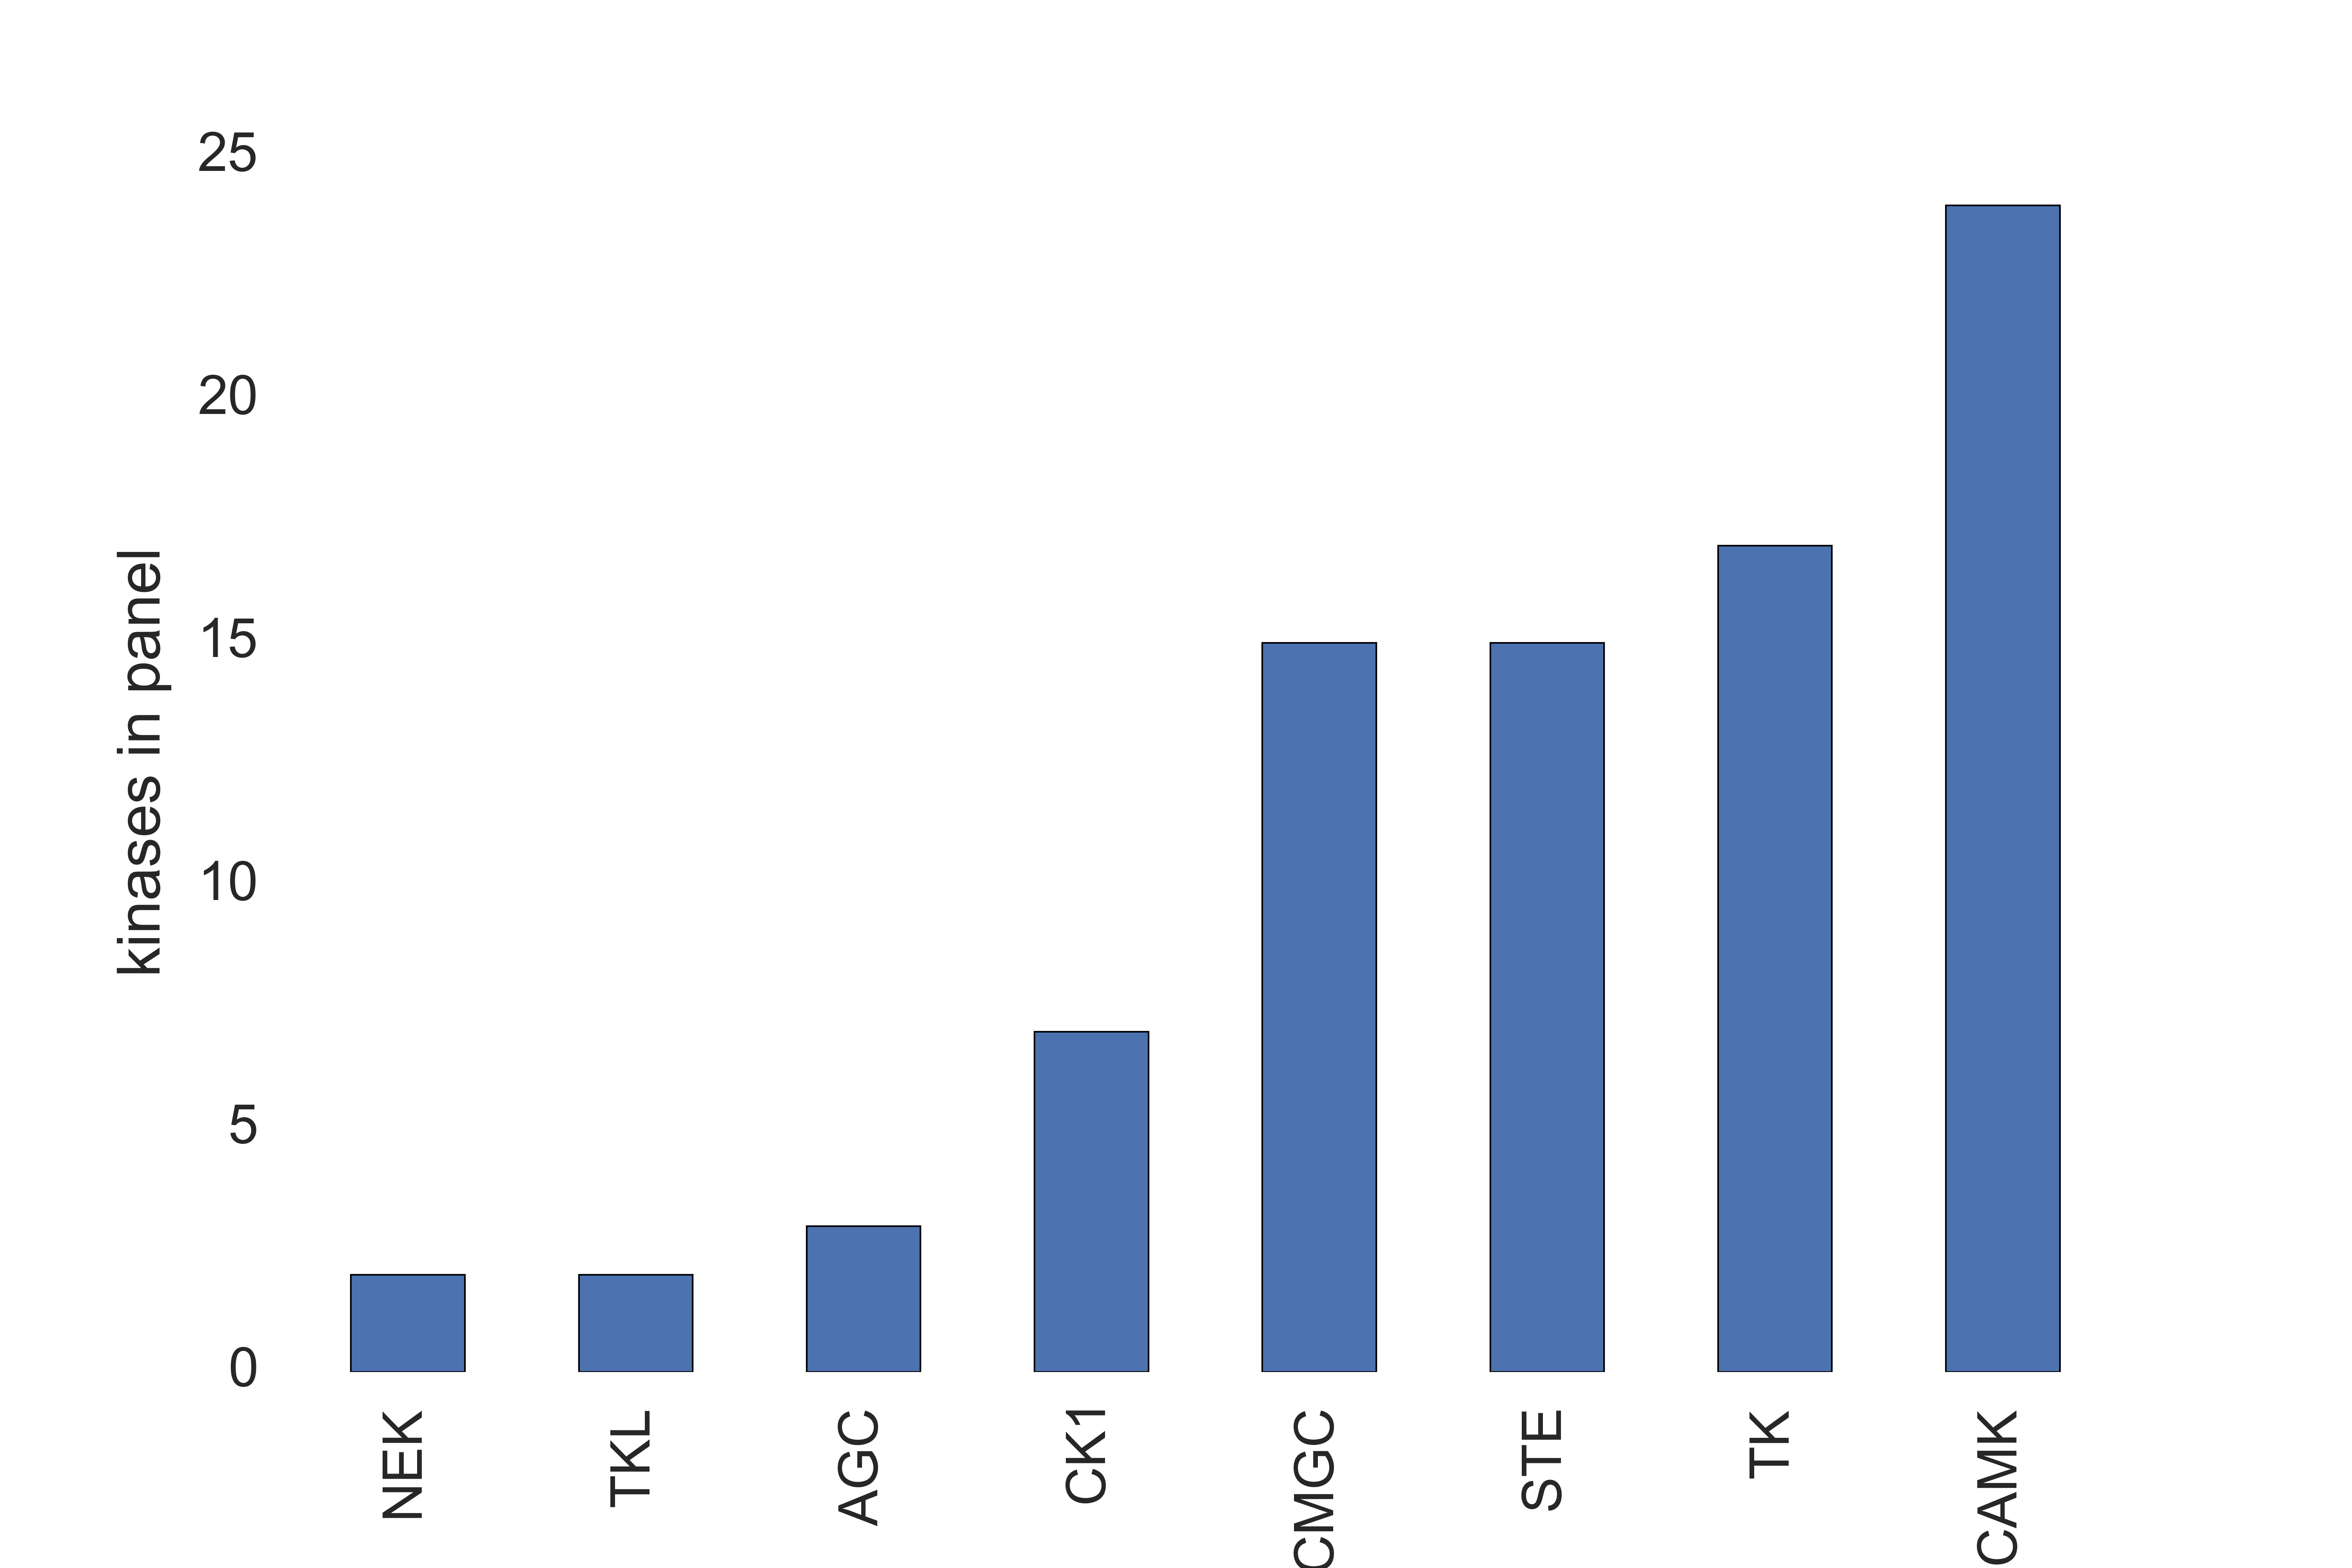
\includegraphics[width=\columnwidth]{figures/ncandidates_byfamily.png}
  \caption{{\bf Distribution of kinases in final expression panel by family.}
   Histogram of the 96 kinases expressed in the expression panel, separated out by kinase family.
   }
  \label{fig:kinases_by_family}
\end{figure}

\subsection{Small-scale kinase expression test in E. coli}

A panel containing the 96 kinase domain constructs selected through our semi-automated method, was tested for expression in E. coli. 
From this initial test, 68 kinase domains expressed successfully (yield of more than 2 ng/$\mu$L ) (Table~\ref{expression_table}).
While the initial panel of 96 kinases was well-distributed across kinase families, the final most highly expressing (yield of more than 100 ng/$\mu$L ) were not as evenly distributed (Figure~\ref{fig:kinome_expression_tree}). 
The 17 most highly expressing kinases all were quite pure with some TEV contaminants still present in Calliper gel images after elution with Imidazole (Figure~\ref{fig:calliper_image}). 

\begin{table*}[]
\centering
\caption{Expression results by kinase}
\label{expression_table}
\footnotesize
\begin{tabular}{p{3.5cm}p{4cm}c}
\toprule
\bf{kinase expressed} & \bf{phosphatase co-expressed} & \bf{concentration (ng/$\mu$l)} \\
\midrule
MK14\_HUMAN\_D0  & Lambda                    & 530                   \\
VRK3\_HUMAN\_D0  & Lambda                    & 506                   \\
GAK\_HUMAN\_D0   & Lambda                    & 485                   \\
CSK\_HUMAN\_D0   & Truncated YopH164         & 469                   \\
VRK1\_HUMAN\_D0  & Lambda                    & 467                   \\
KC1G3\_HUMAN\_D0 & Lambda                    & 422                   \\
FES\_HUMAN\_D0   & Truncated YopH164         & 330                   \\
PMYT1\_HUMAN\_D0 & Lambda                    & 285                   \\
MK03\_HUMAN\_D0  & Lambda                    & 273                   \\
STK3\_HUMAN\_D0  & Lambda                    & 257                   \\
DYR1A\_HUMAN\_D0 & Lambda                    & 256                   \\
KC1G1\_HUMAN\_D0 & Lambda                    & 256                   \\
MK11\_HUMAN\_D0  & Lambda                    & 238                   \\
MK13\_HUMAN\_D0  & Lambda                    & 238                   \\
EPHB1\_HUMAN\_D0 & Truncated YopH164         & 217                   \\
MK08\_HUMAN\_D0  & Lambda                    & 214                   \\
CDK16\_HUMAN\_D0 & Lambda                    & 202                   \\
EPHB2\_HUMAN\_D0 & Truncated YopH164         & 188                   \\
PAK4\_HUMAN\_D0  & Lambda                    & 179                   \\
CDKL1\_HUMAN\_D0 & Lambda                    & 174                   \\
SRC\_HUMAN\_D0   & Truncated YopH164         & 165                   \\
STK16\_HUMAN\_D0 & Lambda                    & 155                   \\
MAPK3\_HUMAN\_D0 & Lambda                    & 141                   \\
PAK6\_HUMAN\_D0  & Lambda                    & 135                   \\
CSK22\_HUMAN\_D0 & Lambda                    & 134                   \\
MERTK\_HUMAN\_D0 & Truncated YopH164         & 126                   \\
PAK7\_HUMAN\_D0  & Lambda                    & 110                   \\
CSK21\_HUMAN\_D0 & Lambda                    & 109                   \\
EPHA3\_HUMAN\_D0 & Truncated YopH164         & 106                   \\
BMPR2\_HUMAN\_D0 & Lambda                    & 106                   \\
M3K5\_HUMAN\_D0  & Lambda                    & 105                   \\
KCC2G\_HUMAN\_D0 & Lambda                    & 100                   \\
E2AK2\_HUMAN\_D0 & Lambda                    & 87                    \\
MK01\_HUMAN\_D0  & Lambda                    & 84                    \\
CSKP\_HUMAN\_D0  & Lambda                    & 76                    \\
CHK2\_HUMAN\_D0  & Lambda                    & 61                    \\
KC1G2\_HUMAN\_D0 & Lambda                    & 57                    \\
DMPK\_HUMAN\_D0  & Lambda                    & 57                    \\
KCC2B\_HUMAN\_D0 & Lambda                    & 53                    \\
FGFR1\_HUMAN\_D0 & Truncated YopH164         & 46                    \\
KS6A1\_HUMAN\_D1 & Lambda                    & 43                    \\
DAPK3\_HUMAN\_D0 & Lambda                    & 30                    \\
STK10\_HUMAN\_D0 & Lambda                    & 28                    \\
KC1D\_HUMAN\_D0  & Lambda                    & 28                    \\
KC1E\_HUMAN\_D0  & Lambda                    & 26                    \\
NEK1\_HUMAN\_D0  & Lambda                    & 25                    \\
CDK2\_HUMAN\_D0  & Lambda                    & 23                    \\
ABL1\_HUMAN\_D0  & Truncated YopH164         & 19                    \\
DAPK1\_HUMAN\_D0 & Lambda                    & 18                    \\
DYRK2\_HUMAN\_D0 & Lambda                    & 18                    \\
HASP\_HUMAN\_D0  & Lambda                    & 17                    \\
FGFR3\_HUMAN\_D0 & Truncated YopH164         & 17                    \\
EPHB3\_HUMAN\_D0 & Truncated YopH164         & 13                    \\
SLK\_HUMAN\_D0   & Lambda                    & 12                    \\
KCC2D\_HUMAN\_D0 & Lambda                    & 12                    \\
NEK7\_HUMAN\_D0  & Lambda                    & 10                    \\
PHKG2\_HUMAN\_D0 & Lambda                    & 10                    \\
VRK2\_HUMAN\_D0  & Lambda                    & 9                     \\
AAPK2\_HUMAN\_D0 & Lambda                    & 8                     \\
AURKA\_HUMAN\_D0 & Lambda                    & 8                     \\
MARK3\_HUMAN\_D0 & Lambda                    & 8                     \\
KAPCA\_HUMAN\_D0 & Lambda                    & 7                     \\
STK24\_HUMAN\_D0 & Lambda                    & 6                     \\
VGFR1\_HUMAN\_D0 & Truncated YopH164         & 4                     \\
KCC4\_HUMAN\_D0  & Lambda                    & 3                     \\
KCC1G\_HUMAN\_D0 & Lambda                    & 2                     \\
KCC2A\_HUMAN\_D0 & Lambda                    & 2                     \\
FAK2\_HUMAN\_D0  & Truncated YopH164         & 2                     \\             
\bottomrule
\end{tabular}
\end{table*}

\begin{figure}[tb]
   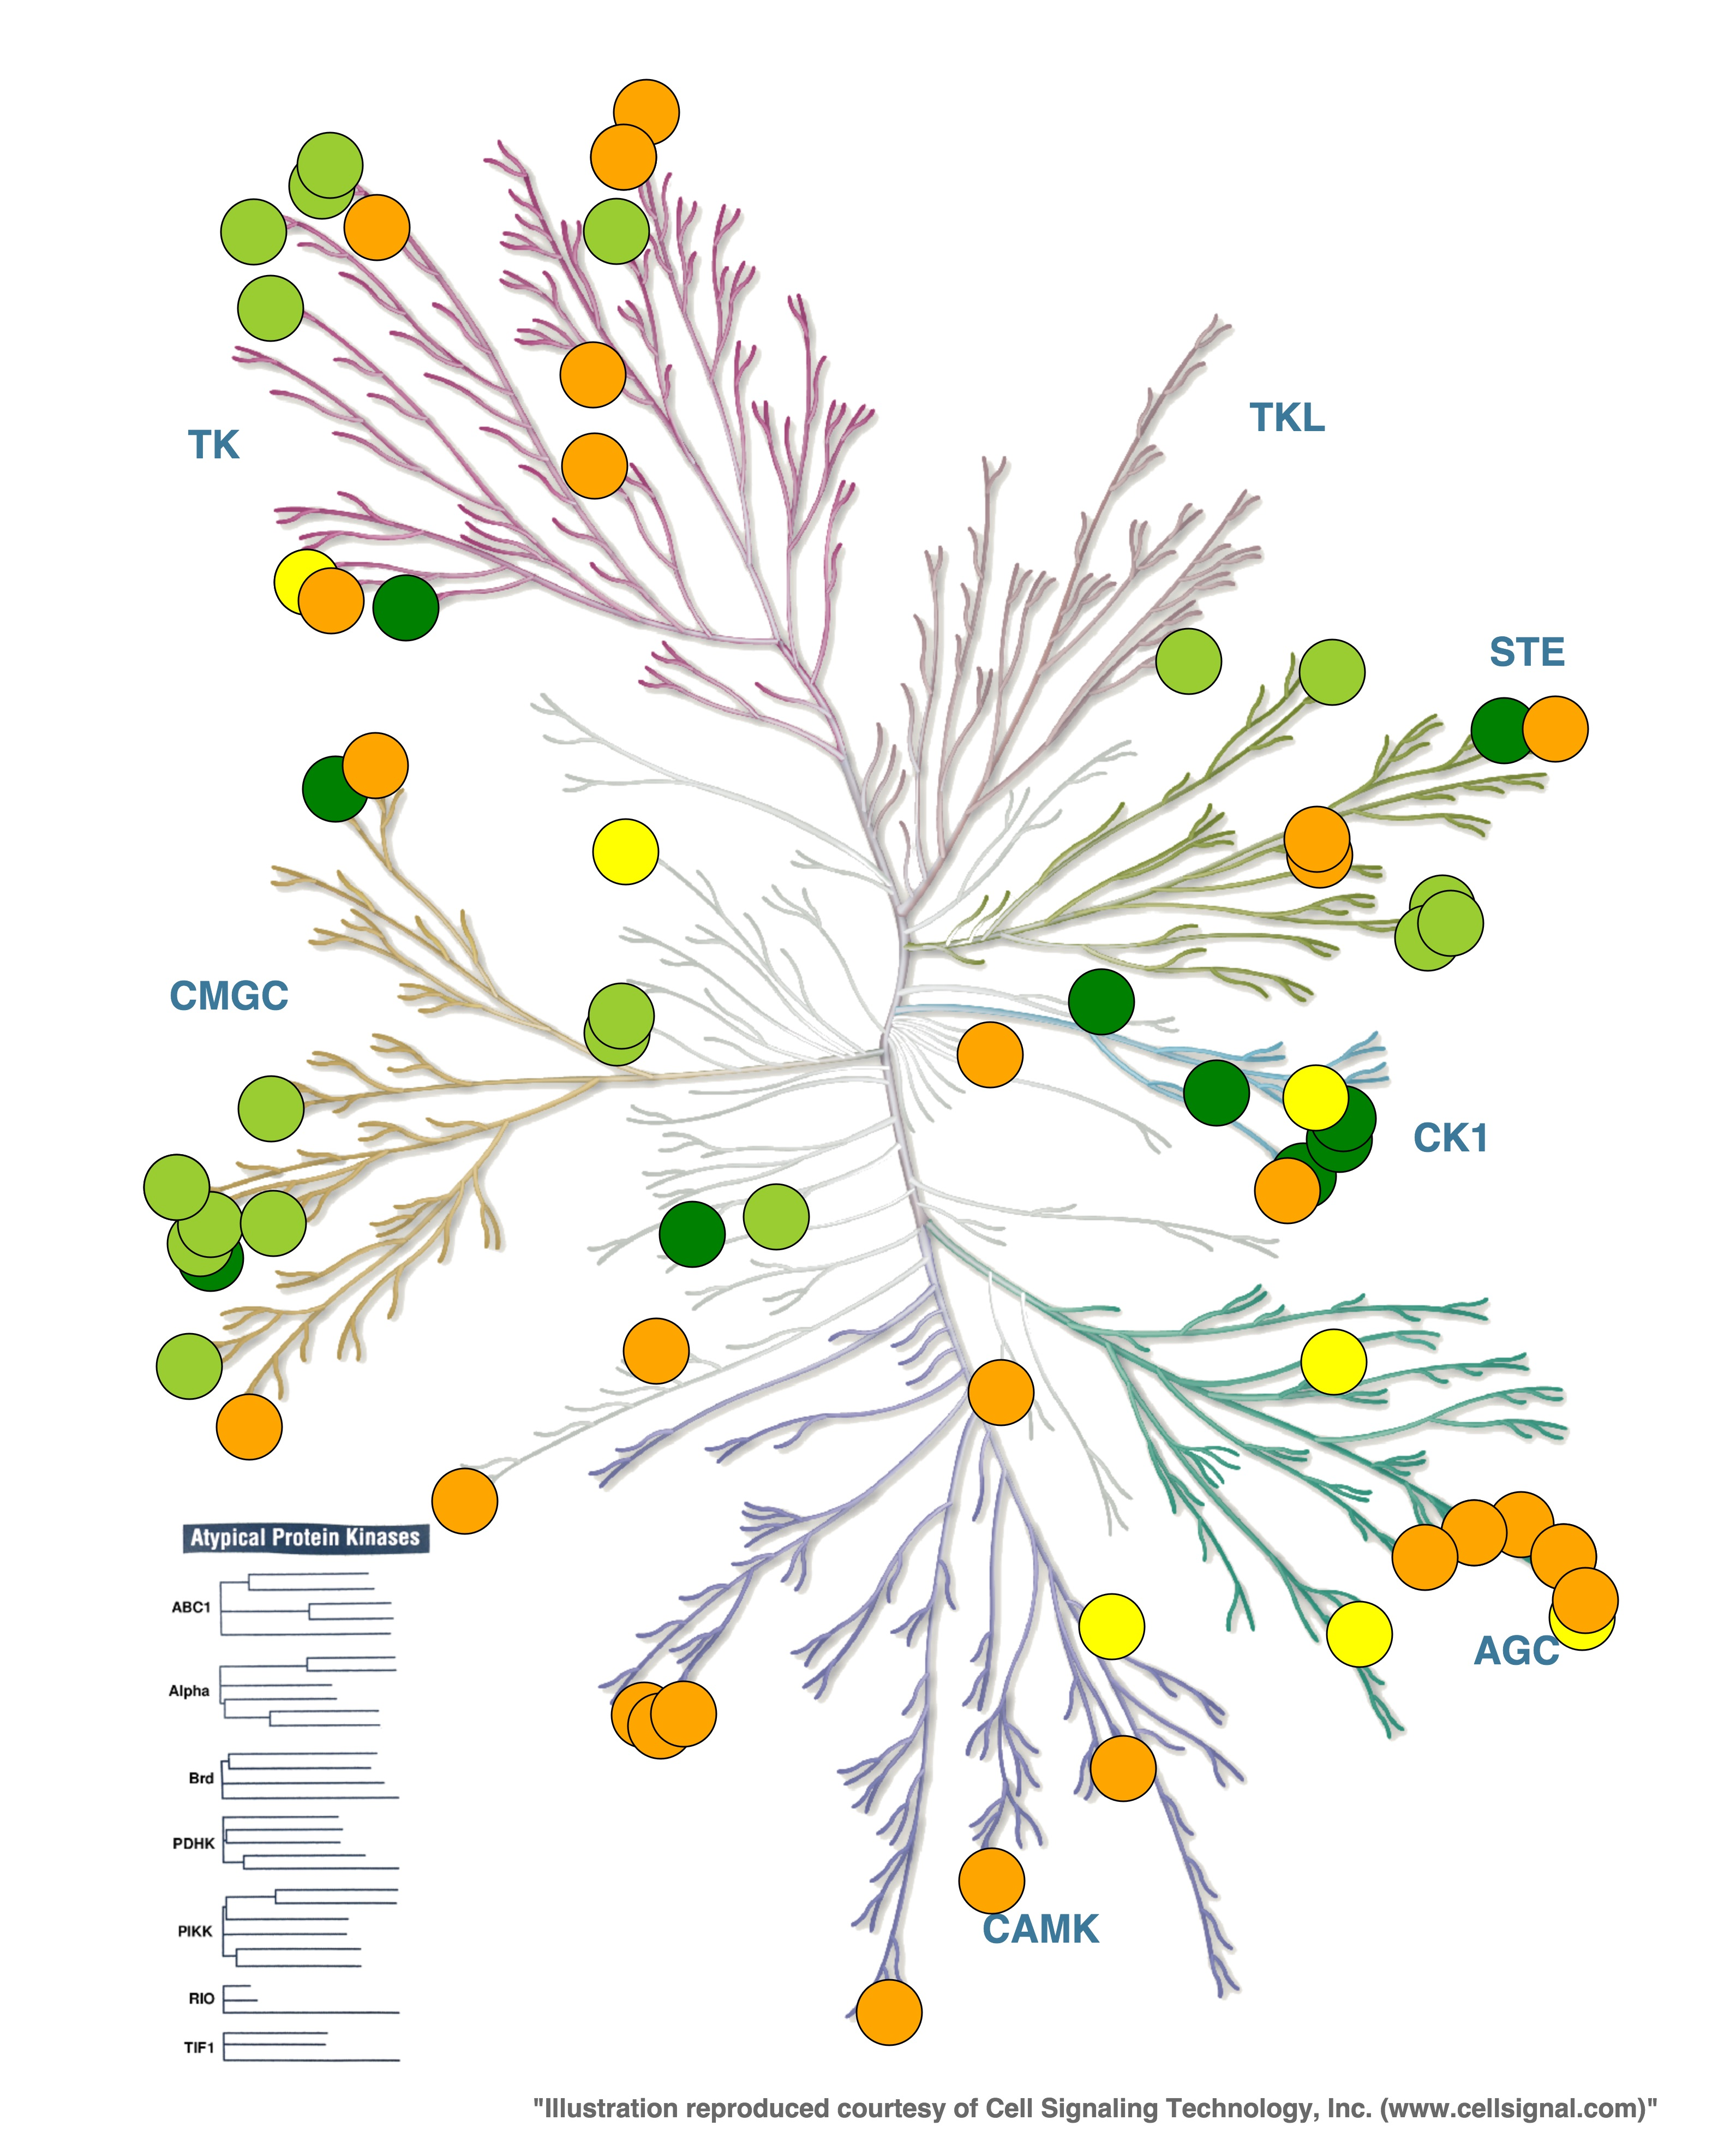
\includegraphics[width=\columnwidth]{figures/kinome_expression.png}
  \caption{{\bf Representation of kinase domain expression results on phylogenetic tree.}
  Dark green circles represent kinases with expression above 250 $ng/ \mu l$.
  Light green circles represent kinases with expression between 100 and 250 $ng/ \mu l$.
  Yellow circles represent kinases with expression between 50 and 100 $ng/ \mu l$.
  Yellow circles represent kinases with any expression up to 50 $ng/ \mu l$.
  Image made with KinMap: \href{http://www.kinhub.org/kinmap}{http://www.kinhub.org/kinmap}. 
   }
  \label{fig:kinome_expression_tree}
\end{figure}

\begin{figure*}[tb]
   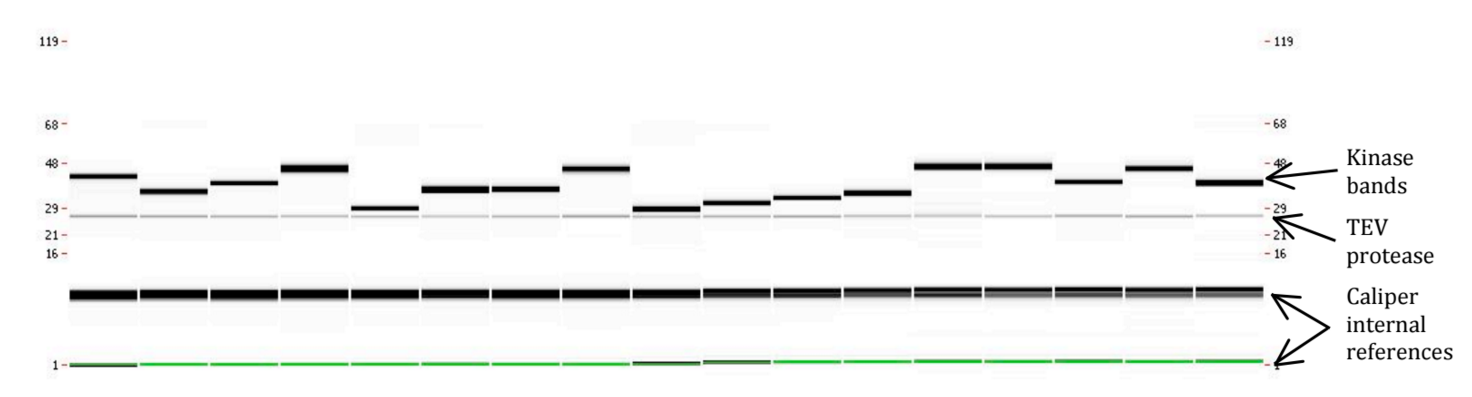
\includegraphics[width=\columnwidth]{figures/calliper_image.png}
  \caption{{\bf Gel image of highest expressing kinases.}
   Calliper gel image of kinases expressing > 200 $ng/ \mu l$.
   }
  \label{fig:calliper_image}
\end{figure*}


%%%%%%%%%%%%%%%%%%%%%%%%%%%%%%%%%%%%%%%%%%%%%%%%%%%%%%%%%%%%%%%%%%%%%%%%%%%%%%%%%%%%%%%%%%%%%%%%%%%%%%
% BIBLIOGRAPHY
%%%%%%%%%%%%%%%%%%%%%%%%%%%%%%%%%%%%%%%%%%%%%%%%%%%%%%%%%%%%%%%%%%%%%%%%%%%%%%%%%%%%%%%%%%%%%%%%%%%%%%

\bibliographystyle{prsty} 
\bibliography{ms.bib}

\end{document}
